\clearpage
\section{Modelling a Single Data Set}


\begin{figure}[htb]
\begin{center}
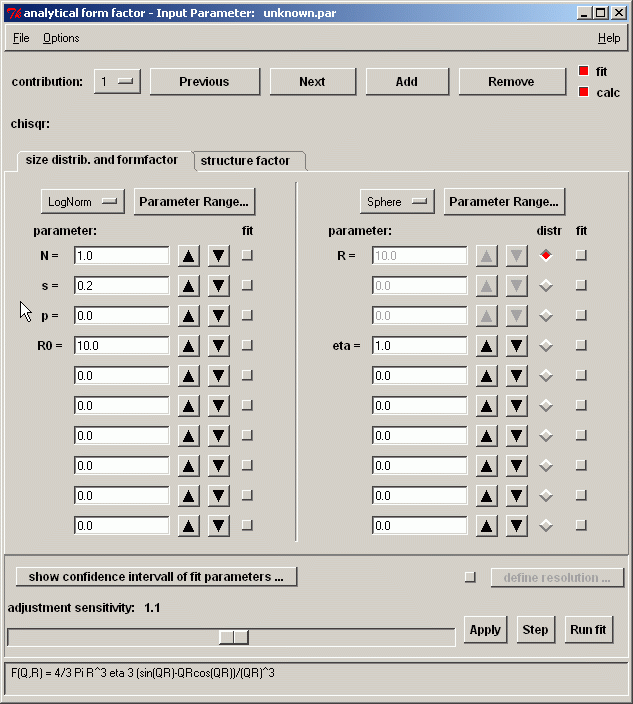
\includegraphics[width=0.45\textwidth,height=0.55\textwidth]{analyticalMenu1.png}
~\hspace{3mm}
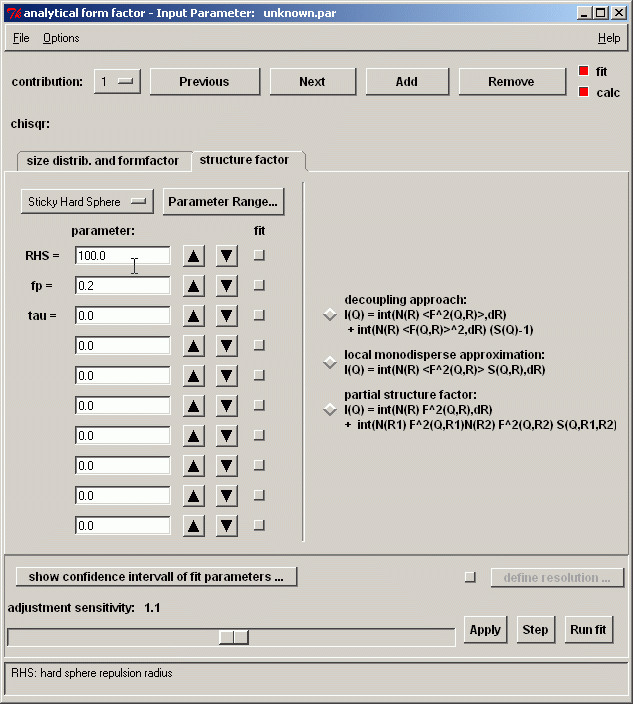
\includegraphics[width=0.45\textwidth,height=0.55\textwidth]{analyticalMenu2.png}
\end{center}
\caption{A user interface to choose between the number of scattering
objects and to define parameter for each of them.}
 \label{analyticalMenu}
\end{figure}


\begin{figure}[htb]
\begin{center}
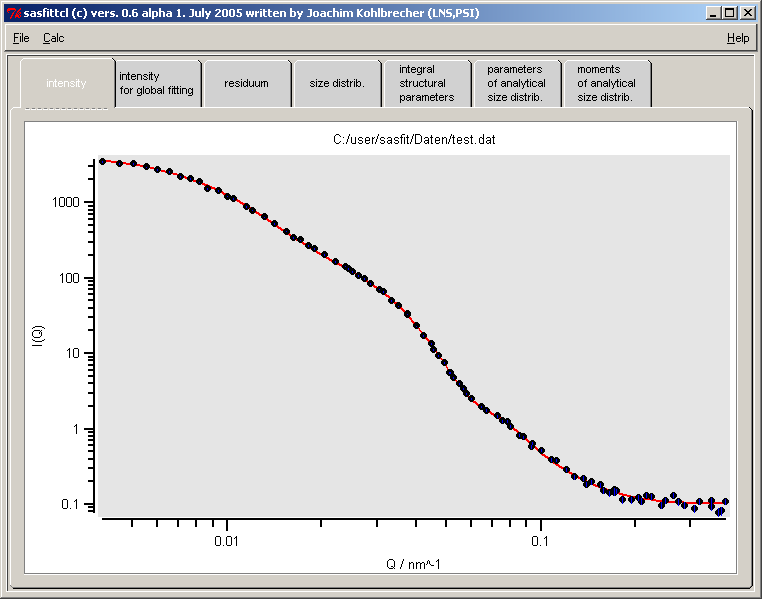
\includegraphics[width=0.75\textwidth,height=0.55\textwidth]{sasfit_1.png}
\end{center}
\caption{} \label{fig1}
\end{figure}

\begin{figure}[htb]
\begin{center}
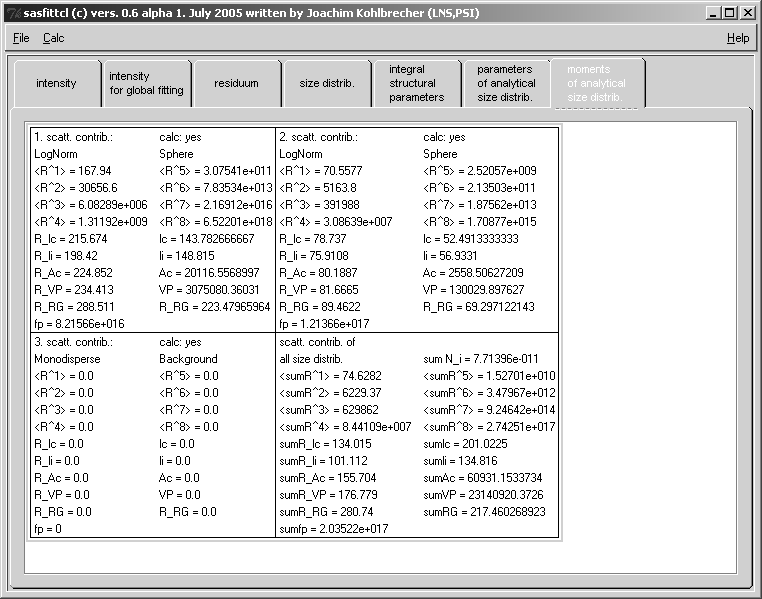
\includegraphics[width=0.45\textwidth,height=0.3\textwidth]{tab1.png}
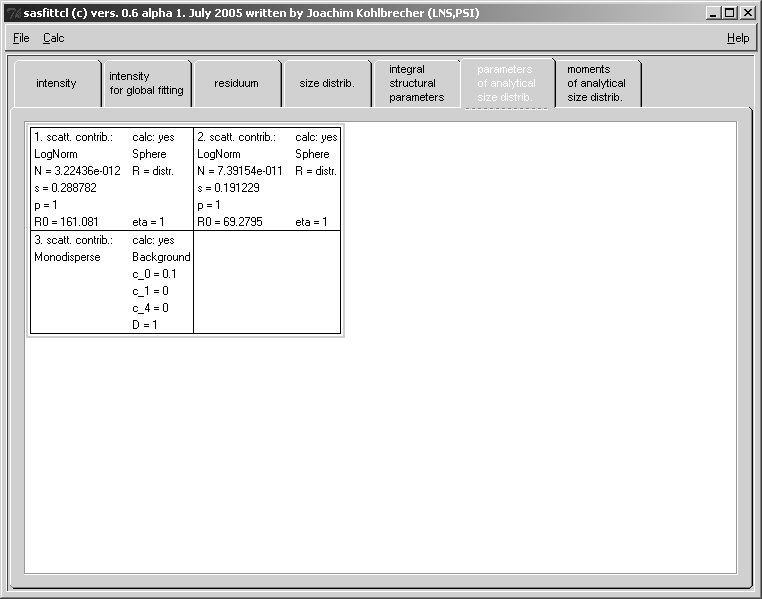
\includegraphics[width=0.45\textwidth,height=0.3\textwidth]{tab2.png}
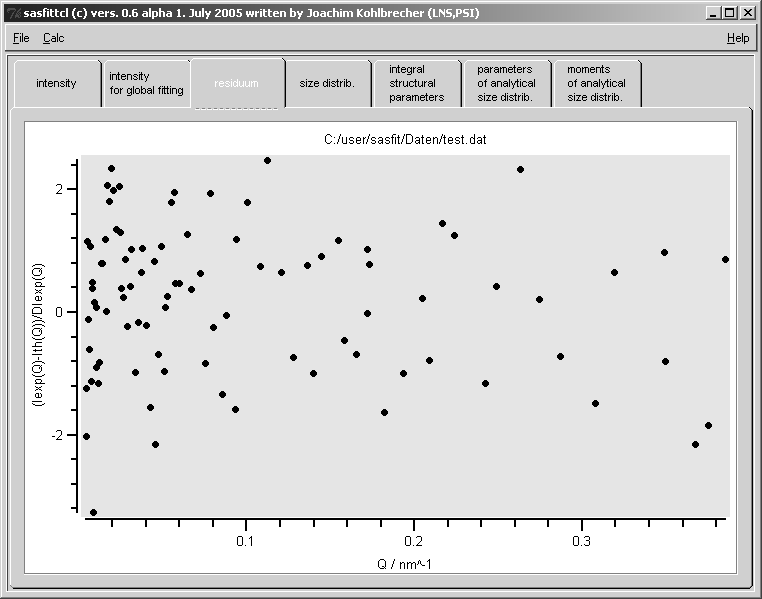
\includegraphics[width=0.45\textwidth,height=0.3\textwidth]{tab3.png}
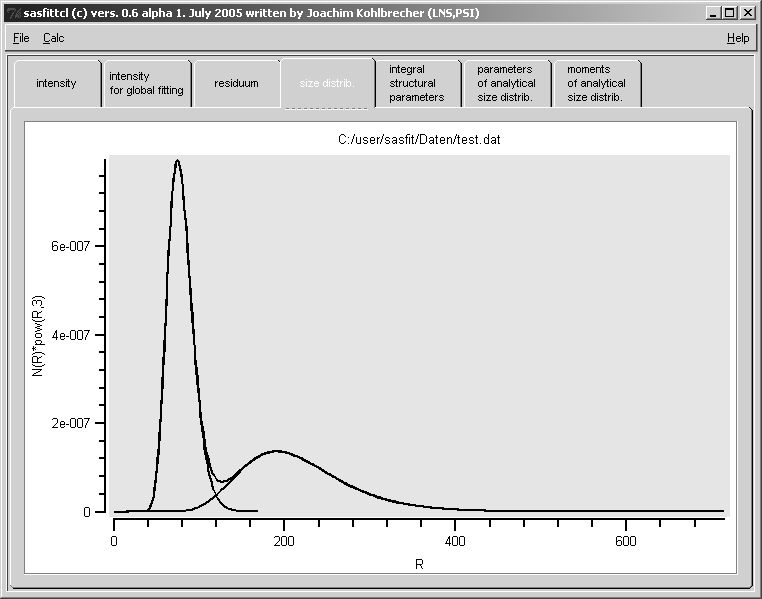
\includegraphics[width=0.45\textwidth,height=0.3\textwidth]{tab4.png}
\end{center}
\caption{} \label{tabs}
\end{figure}
